\documentclass[10pt]{beamer}

%%%
% PREAMBLE FOR THIS DOC 
%%%
%https://tex.stackexchange.com/questions/68821/is-it-possible-to-create-a-latex-preamble-header
\usepackage{/Users/miw267/Repos/latex_preamble/beamer_preamble}


%%% TRY TO RESHOW TOC AT EACH SECTION START (with current section highlighted)
% Reference: https://tex.stackexchange.com/questions/280436/how-to-highlight-a-specific-section-in-beamer-toc
\newcommand\tocforsect[2]{%
  \begingroup
  \edef\safesection{\thesection}
  \setcounter{section}{#1}
  \tableofcontents[#2,currentsection]
  \setcounter{section}{\safesection}
  \endgroup
}


%%%% HERES HOW TO DO IT CORRECTLY
% FIRST IN .STY FILE, DO
%\usetheme[sectionpage=none]{metropolis}
% THEN AT EACH SECTION DO
%\begin{frame}{Outline}
%  \tableofcontents[currentsection]	
%\end{frame}



%\setbeamertemplate{navigation symbols}{}
%\setbeamertemplate{footline}[frame number]{}

%%% SPECIAL FOR THIS DOC
\usetikzlibrary{arrows.meta}




%%%
% AGENDA TOPICS
%%%
\agendatopic[congruence]{Congruence mod n}
\agendatopic[review]{Review of relations}
\agendatopic[equivalence]{Equivalence relations}



%%%
% DOCUMENT
%%%

\begin{document}

%\maketitle

%% Title page frame
%\begin{frame}
%    \titlepage 
%\end{frame}





\title{09/25/2026: Equivalence Relations}
\author{CSCI 246: Discrete Structures}
\date{Textbook reference: Sec 15, Scheinerman}

\begin{frame}
    \titlepage 
\end{frame}


\begin{frame}


\begin{myyellowbox}[title=Today's Agenda]
\begin{itemize}
	\item Quiz ($\approx$ 15 mins) 
	\item Mini-lecture ($\approx$ 20 mins)
	\item Group exercises ($\approx$ 15 mins)
\end{itemize}	
\end{myyellowbox}

\end{frame}


\begin{frame}

\begin{myredbox}[title=Quiz logistics]
	
\begin{itemize}
	\item Please put your last name on the back.
	\item Please put your first and last name on the front.
\end{itemize}
\end{myredbox}

\vfill 

\begin{mygreenbox}[title=Reminder]
Please see me if you think your quiz was misgraded.
\end{mygreenbox}



\end{frame} 

\begin{frame}{Weekly Quiz \#4}

\begin{enumerate}
	\item (Sets.) How many subsets does the set $A=\set{1,2,3}$ have? Justify your answer.
	\item (Quantifiers.) For each sentence below, write the negation of the sentence, but place the $\lnot$ symbol as far to the right as possible. Then rewrite the negation in English.
    \begin{itemize}    
        \item[a.] $\forall x \in \mathbb{Z}, x \text{ is odd.}$
        \item[b.] $\forall x \in \mathbb{Z}, x<0.$  
  	\end{itemize}
  	\item (Set Operations.)  How many integers in the range 1 to 1000 (inclusive) are divisible by 2 or by 5?  Justify your answer.  \textit{Hint:} Use the proposition giving the size of a union of sets.
\end{enumerate}
\vfill 
\begin{mygreenbox}[title=Proposition: Size of a Union]
Let $A$ and $B$ be sets.  Then
\[|A \cup B|  = |A| + |B| - |A \cap B| \]
\end{mygreenbox}
\end{frame}



\agendaframe{congruence}




\begin{frame}{Congruence mod $n$}
 \small 
\begin{mygreenbox}[title=Definition]
Let $n$ be a positive integer.  We say that integers $x$ and $y$ are \textbf{congruent modulo n}, and we write 
\[x \equiv y \quad \text{(mod $n$)} \]
if $n | (x-y)$.
\end{mygreenbox}
\vfill 
\pause 
\colorbox{red!30}{\textbf{Remark.}} In other words, $x \equiv y \quad \text{(mod $n$)}$ if and only if $x$ and $y$ differ by a multiple of $n$.
%\textbf{Remark.} For intuition, note  that $x \equiv y$ (mod $n$) if $x$ and $y$ have the same remainder after dividing by $n$.  For example, $6 \equiv 1$ (mod 5).
\vfill 
\pause 
\colorbox{green!30}{\textbf{Example.}} 
%
\only<3-5>{
\begin{align*}
\only<3-5>{3 & \equiv 13 \; \text{(mod $5$)}?} && \only<4-5>{\text{Yes, because $3-13=-10$ is a multiple of 5}} 
\end{align*}
}
%
\only<5>{
%\begin{center}
%\begin{tikzpicture}[xscale=0.52, yscale=0.5]
%  \draw[->,thick] (-3.6,0) -- (15.6,0);
%  \foreach \x in {-3,...,15}{ \draw (\x,0.12) -- (\x,-0.12); }
%  \foreach \x in {-3,-1,1,2,4,5,6,7,9,10,11,12,14,15}{ \node[below,font=\tiny,black!55] at (\x,-0.16) {$\x$}; }
%  \foreach \x in {-2,3,8,13}{ \fill[red!80!black] (\x,0) circle (2.6pt);
%                              \node[below,font=\scriptsize\bfseries,red!80!black] at (\x,-0.18) {$\x$}; }
%  \foreach \a/\b in {-2/3,3/8,8/13}{
%     \draw[->,thick,red!80!black] (\a,0.12) to[bend left=55] node[above,font=\tiny]{$+5$} (\b,0.12); }
%\end{tikzpicture}
%\end{center}
\begin{center}
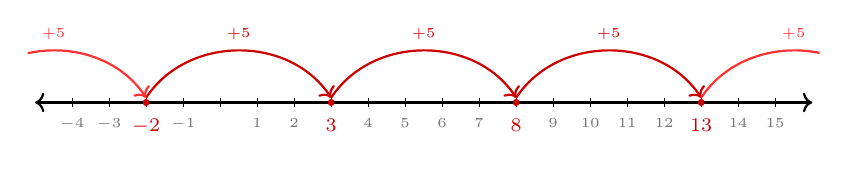
\begin{tikzpicture}[xscale=0.47, yscale=0.5]
  \draw[<->,thick] (-5.0,0) -- (16.0,0);
  \foreach \x in {-4,...,15}{ \draw (\x,0.12) -- (\x,-0.12); }
  \foreach \x in {-4,-3,-1,1,2,4,5,6,7,9,10,11,12,14,15}{ \node[below,font=\tiny,black!55] at (\x,-0.16) {$\x$}; }
  \foreach \x in {-2,3,8,13}{ \fill[red!80!black] (\x,0) circle (2.6pt);
                              \node[below,font=\scriptsize\bfseries,red!80!black] at (\x,-0.18) {$\x$}; }
  % all five hops are the same +5 arc; the outer two run off the edge
  \begin{scope}
    \clip (-5.2,-0.9) rectangle (16.2,1.9);
    \foreach \a/\b in {-2/3}{
       \draw[->,thick,red!80!black] (\a,0.12) to[bend left=55] node[above,font=\tiny]{$+5$} (\b,0.12); }
      \foreach \a/\b in {3/8,8/13}{
       \draw[->,thick,red!80!black] (\a,0.12) to[bend left=55] node[above,font=\tiny]{$+5$} (\b,0.12); }
    \foreach \a/\b in {-7/-2,13/18}{
       \draw[->,thick,red!80!white] (\a,0.12) to[bend left=55] node[above,font=\tiny]{$+5$} (\b,0.12); }
  \end{scope}
\end{tikzpicture}
\end{center}
}
%
\only<6-8>{
\begin{align*}
\only<6-8>{4 & \equiv 4 \; \text{(mod $5$)}?} && \only<7-8>{\text{Yes, because $4-4=0$ is a multiple of 5}} 
\end{align*}
}
%
\only<8>{
\begin{center}
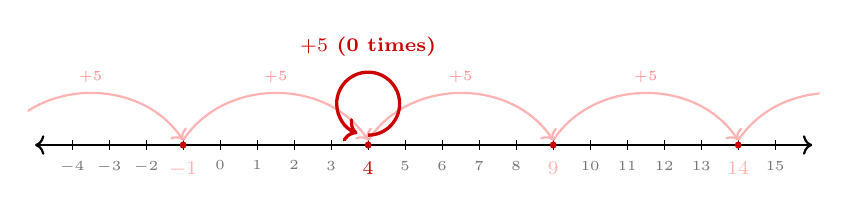
\begin{tikzpicture}[xscale=0.47, yscale=0.5]
  \draw[<->,thick] (-5.0,0) -- (16.0,0);
  \foreach \x in {-4,...,15}{ \draw (\x,0.12) -- (\x,-0.12); }
  \foreach \x in {-4,-3,-2,0,1,2,3,5,6,7,8,10,11,12,13,15}{ \node[below,font=\tiny,black!55] at (\x,-0.16) {$\x$}; }
  \foreach \x in {-1,9,14}{ \fill[red!80!black] (\x,0) circle (2.6pt);
                              \node[below,font=\scriptsize\bfseries,red!30!white] at (\x,-0.18) {$\x$}; }
   \foreach \x in {4}{ \fill[red!80!black] (\x,0) circle (2.6pt);
                              \node[below,font=\scriptsize\bfseries,red!80!black] at (\x,-0.18) {$\x$}; }
  \begin{scope}
    \clip (-5.2,-0.9) rectangle (16.2,2.6);
    \foreach \a/\b in {-6/-1,-1/4,4/9,9/14,14/19}{
       \draw[->,thick,red!30!white] (\a,0.12) to[bend left=55] node[above,font=\tiny,red!45!white]{$+5$} (\b,0.12); }
  \end{scope}
  % zero hops: you are already there
  \draw[->,very thick,red!80!black] (4,0.25) arc (-90:250:0.85 and 0.8);
  \node[font=\scriptsize\bfseries,red!80!black] at (4,2.5) {$+5$ (0 times)};
\end{tikzpicture}
\end{center}
}
\only<9-11>{
\begin{align*}
\only<9-11>{16 & \, \equiv \,  3 \; \text{(mod $5$)}?} && \only<10-11>{\text{NO, because $16-3=13$ is not a multiple of 5}} 
\end{align*}
}
\only<11>{

\begin{center}
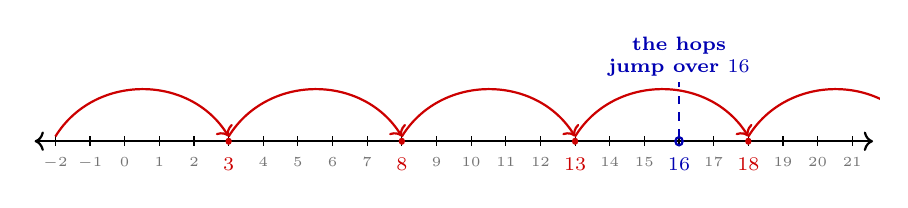
\begin{tikzpicture}[xscale=0.44, yscale=0.5]
  \draw[<->,thick] (-2.6,0) -- (21.6,0);
  \foreach \x in {-2,...,21}{ \draw (\x,0.12) -- (\x,-0.12); }
  \foreach \x in {-2,-1,0,1,2,4,5,6,7,9,10,11,12,14,15,17,19,20,21}{
      \node[below,font=\tiny,black!55] at (\x,-0.16) {$\x$}; }
  \foreach \x in {3,8,13,18}{ \fill[red!80!black] (\x,0) circle (2.6pt);
                              \node[below,font=\scriptsize\bfseries,red!80!black] at (\x,-0.18) {$\x$}; }
  % 16 is not in the class
  \draw[blue!70!black,thick] (16,0) circle (3pt);
  \node[below,font=\scriptsize\bfseries,blue!70!black] at (16,-0.18) {$16$};
  \draw[blue!70!black,dashed] (16,0.1) -- (16,1.5);
  \node[font=\scriptsize\bfseries,blue!70!black,align=center] at (16,2.15) {the hops\\ jump over $16$};
  \begin{scope}
    \clip (-2.8,-0.9) rectangle (21.8,1.55);
    \foreach \a/\b in {-2/3,3/8,8/13,13/18,18/23}{
       \draw[->,thick,red!80!black] (\a,0.12) to[bend left=55] node[above,font=\tiny]{$+5$} (\b,0.12); }
  \end{scope}
\end{tikzpicture}
\end{center}

}


\end{frame}



\begin{frame}{Application: hashing features in machine learning}
\footnotesize

\begin{mygreenbox}[title=Problem]
A text model needs a \textbf{feature index} for every word.  The vocabulary is unbounded,
but the feature vector has \textbf{fixed} length $m$.
\end{mygreenbox}

\pause
\vspace{-.2cm}
\begin{mybluebox}[title=The hashing trick]
Pick any hash function $h$ (which converts the words to integers) and use $\;\text{index}(w) = h(w) \bmod m$.  With $m=5$:
\vspace{-0.4em}
\begin{center}\scriptsize
\begin{tabular}{l r c l}
\textbf{word} & $h(w)$ & $h(w) \bmod 5$ & \textbf{bucket} \\
\hline
\texttt{"cat"} & $918273$ & $3$ & \red{$[3]$} \\
\texttt{"dog"} & $460815$ & $0$ & $[0]$ \\
\texttt{"the"} & $203948$ & $3$ & \red{$[3]$ \; collision!} \\
\texttt{"run"} & $771236$ & $1$ & $[1]$ \\
\end{tabular}
\end{center}
\end{mybluebox}

\only<3>{
\vspace{0.4em}
\begin{myredbox}[title=The connection]
\qq{Same bucket} \emph{is} \alert{congruence mod $m$}: the $m$ buckets are its equivalence
classes, and a \textbf{collision} is two words in one class.  
\end{myredbox}
}
 

\only<4->{
\vspace{-.2cm}
\begin{myyellowbox}[title=Advantages]
\begin{itemize}
\item<4-> \textbf{No dictionary.} The mapping isn't stored anywhere; it's a formula. "cat" hashes to 918273, so bucket $918273 \bmod 5 = 3$, every time,  on every machine. Zero bytes of lookup table.
\vspace{-.2cm}
\item<5> \textbf{Fixed memory.} You choose $m$ up front and that's the whole model width. At $m = 2^{20}$ that's 4.2 MB of float32 weights, regardless of whether you've seen a thousand words or ten million.
\end{itemize}
\end{myyellowbox}
}



\end{frame}


\begin{frame}{Application: Public-Key Cryptography}
\footnotesize 
\begin{figure}[ht]
        \centering
        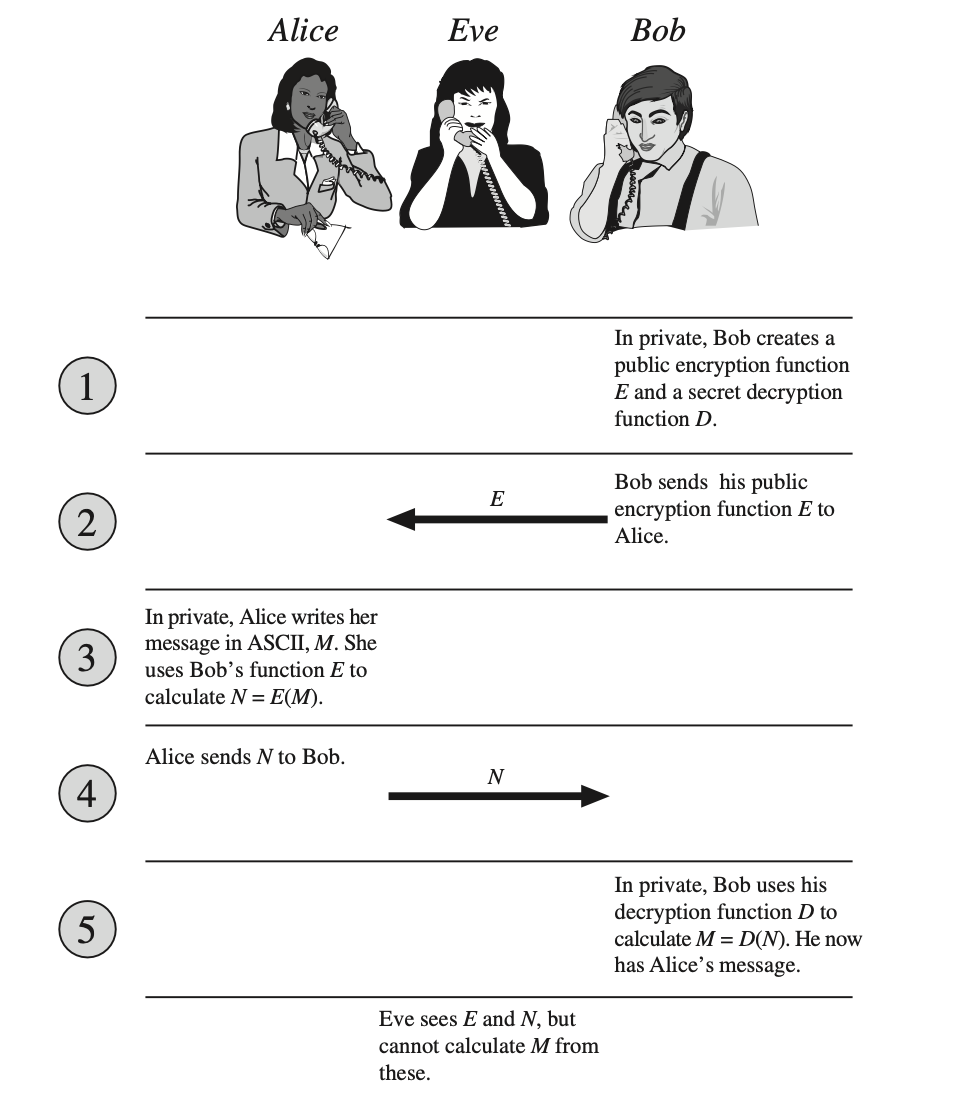
\includegraphics[width=.65\textwidth]{images/cryptography}
   		 %\caption{Median Score = 4/4 (100\%)}
\end{figure}
\vfill 
\end{frame}





%
%\begin{frame}{Applications of congruence mod $n$}
%
%\begin{itemize}
%	\item \textbf{Cryptography}: RSA, Diffie–Hellman, elliptic curve cryptography — all depend on modular arithmetic.
%	\item \textbf{Computer science}: Hashing, checksums, random number generators, error detection codes.
%	\item \textbf{Number theory}: Solving Diophantine equations, proving divisibility, Fermat’s little theorem, Chinese Remainder Theorem.
%	\item \textbf{Everyday math}: Clocks, calendars, cyclic patterns.
%\end{itemize}
%
%
%	
%\end{frame}


\agendaframe{review}

%
%\begin{frame}{Review: Relations}
% 
%\small 
% 
%\begin{mygreenbox}[title=Definition (Scheinerman Def 14.1)]
%A \textbf{relation} is a set of ordered pairs.
%\end{mygreenbox}	
%\vfill 
%\pause 
%
%\begin{mybluebox}[title=Example]
%\begin{itemize}
%\item Let $P$ be a set of people. Let $C$ be a set of cities.	
%\item Define the relation $R \subseteq P \times C$ by 
%\[ R = \set{(p,c) : \text{ person $p$ has lived in city $c$.}} \] 
%\end{itemize}
%
%
%\begin{center}
%\resizebox{0.45\textwidth}{!}{%
%\begin{tikzpicture}[>={Stealth[length=8pt,width=6pt]}, node distance=3mm, thick]
%
%  % People nodes
%  \node (Mike) {\Large Mike};
%  \node[below=of Mike] (Madhav) {\Large Madhav};
%  % Ellipse around P
%  \node[draw, ellipse, fit=(Mike)(Madhav), inner sep=1mm] (P) {};
%  \node at (P.north) [above] {\Large $P$};
%
%  % City nodes
%  \node[right=5cm of Mike] (Bozeman) {\Large Bozeman};
%  \node[above=of Bozeman] (Jacksonville) {\Large Jacksonville, FL};
%  \node[above=of Jacksonville] (Seattle) {\Large Seattle};
%  \node[below=of Bozeman] (Rockfield) {\Large Delhi, India};
%  \node[below=of Rockfield] (Butte) {\Large Paris, France};
%  \node[below=of Butte] (Billings) {\Large Billings};
%  % Ellipse around C
%  \node[draw, ellipse, fit=(Bozeman)(Jacksonville)(Seattle)(Rockfield)(Butte)(Billings),
%        inner sep=1mm] (C) {};
%  \node at (C.north) [above] {\Large $C$};
%
%  % Arrows from Mike
%  \draw[->] (Mike.east) -- (Bozeman.west);
%  \draw[->] (Mike.east) -- (Seattle.west);
%  \draw[->] (Mike.east) -- (Jacksonville.west);
%
%  % Arrows from Megan
%  \draw[->] (Madhav.east) -- (Bozeman.west);
%  \draw[->] (Madhav.east) -- (Rockfield.west);
%  \draw[->] (Madhav.east) -- (Butte.west);
%
%\end{tikzpicture}
%}
%\end{center}
%\end{mybluebox}
%
%\end{frame}


\begin{frame}{Review: Relations}

\small

\begin{columns}[T,onlytextwidth]
\begin{column}{0.62\textwidth}
\begin{mygreenbox}[title=Definition (Scheinerman Def 14.1)]
A \textbf{relation} is a set of ordered pairs.
\end{mygreenbox}	

\vspace{-0.2cm} 
\pause

\begin{mybluebox}[title=Example]
 Let $P$ be a set of people. Let $C$ be a set of cities. \pause  Define the relation $R \subseteq P \times C$ by 
\vspace{-0.2cm}
\[ R = \set{(p,c) : \text{ person $p$ has lived in city $c$.}} \] 

\pause 
\begin{center}
\resizebox{0.6\textwidth}{!}{%
\begin{tikzpicture}[>={Stealth[length=8pt,width=6pt]}, node distance=3mm, thick]

  % People nodes
  \node (Mike) {\Large Mike};
  \node[below=of Mike] (Madhav) {\Large Madhav};
  \node[above=of Mike] (pdots1) {\Large $\vdots$};
  \node[below=of Madhav] (pdots2) {\Large $\vdots$};
  
  % Ellipse around P
  \node[draw, ellipse, fit=(pdots1)(pdots2), inner sep=5mm] (P) {};
  \node at (P.north) [above] {\Large $P$};

  % City nodes
  \node[right=5cm of Mike] (Bozeman) {\Large Bozeman};
  \node[above=of Bozeman] (Jacksonville) {\Large Jacksonville, FL};
  \node[above=of Jacksonville] (Seattle) {\Large Seattle};
  \node[below=of Bozeman] (Rockfield) {\Large Delhi, India};
  \node[below=of Rockfield] (Butte) {\Large Paris, France};
  \node[below=of Butte] (Billings) {\Large Mexico City};
   \node[above=of Seattle] (cdots1) {\Large $\vdots$};
    \node[below=of Billings](cdots2){\Large $\vdots$};
    
  % Ellipse around C
  \node[draw, ellipse, fit=(Seattle)(Billings),
        inner sep=10mm] (C) {};
  \node at (C.north) [above] {\Large $C$};

  % Arrows from Mike
  \draw[->] (Mike.east) -- (Bozeman.west);
  \draw[->] (Mike.east) -- (Seattle.west);
  \draw[->] (Mike.east) -- (Jacksonville.west);

  % Arrows from Megan
  \draw[->] (Madhav.east) -- (Bozeman.west);
  \draw[->] (Madhav.east) -- (Rockfield.west);
  \draw[->] (Madhav.east) -- (Butte.west);

\end{tikzpicture}
}
\end{center}
\end{mybluebox}

\end{column}

\begin{column}{0.36\textwidth}
\onslide<5->%
\only<5->{\begin{myyellowbox}[title=Poll]
How is a \textbf{relation} different from a \textbf{function}?
\end{myyellowbox}}

\vfill
\only<6->{\begin{mygreenbox}[title=Solution]
\only<6->{
\begin{itemize}
\item For a \textbf{function}, each input has \alert{only one} output.
\item For a \textbf{relation}, an input can have \alert{more than one} output.
\end{itemize}
}
\vspace{0.3em}
\only<7->{So a relation is a \textbf{generalization} of a function.}
\end{mygreenbox}
}
\end{column}
\end{columns}

\end{frame}

\begin{frame}{Review: Properties of Relations}
\small
\only<9>{\footnotesize}
\colorbox{yellow!30}{\textbf{Goal.}} Let's state the three main properties of relations and try to give an example/non-example for each.
\pause 

 \begin{mygreenbox}[title=Definition]
Suppose that $R$ is a relation on a set $A$.
\begin{enumerate}
	\item \only<3-4,9>{The relation $R$ is \textbf{reflexive} on $A$ if $a\,R\,a$ for all $a \in A$.}
	\item  \only<5-6,9>{The relation $R$ is \textbf{symmetric} on $A$ if, whenever $a\,R\,b$, then also $b\,R\,a$.}
	\item \only<7-8,9>{The relation $R$ is \textbf{transitive} on $A$ if, whenever $a\,R\,b$ and $b\,R\,c$, then also $a\,R\,c$.}
\end{enumerate}
\end{mygreenbox}
\vfill 
\begin{mybluebox}[title=Examples]
Let $A$ be the set of people.  
\begin{enumerate}
		\item \only<4,9>{\textbf{Reflexivity.} \pause The \texttt{lives-in-the-same-city-as} relation is reflexive, but the \texttt{parent-of} relation is not.} 
	\vspace{-.2cm} 
	\item \only<6,9>{\textbf{Symmetry.} \pause The \texttt{friends-of} relation is symmetric (usually -- 
\includegraphics[height=1em]{images/eek}), but \texttt{parents-of} relation is not.}
	\item \only<8,9>{\textbf{Transitivity.} \pause The \texttt{is-in-the-same-family} relation is transitive, but the \texttt{parent-of} relation is not.}
\end{enumerate}
	
\end{mybluebox}

\end{frame}

\agendaframe{equivalence}



\begin{frame}{Equivalence Relations: A mathematical notion of \alert{sameness}}
\pause 
\begin{myredbox}[title=Definition]
An \textbf{equivalence relation} is a relation that is
\begin{enumerate}
\item Reflexive \greencheck
\item Symmetric \greencheck
\item Transitive \greencheck
\end{enumerate}
\end{myredbox}	

\vfill 
\pause 
\colorbox{yellow!30}{\textbf{Poll.}} Why these three properties?
 \vfill 
\pause 
\colorbox{green!30}{\textbf{Solution.}}
\begin{enumerate}
\item \textit{Reflexivity.}  \pause Without this, you’d have a notion of \qq{sameness} that excludes the most obvious case.
\item \textit{Symmetry.} \pause Sameness should go both ways. Otherwise you’d have a strange, one-sided notion of \qq{sameness.}
\item \textit{Transitivity.} \pause \qq{Sameness} should spread consistently along chains of relations. (It would be weird if $a$ was the same as $b$, and $b$ was the same as $c$, but $c$ wasn't the same as $a$.) 
\end{enumerate}

\end{frame}



\begin{frame}{Equivalence relations: Example}
\small


\only<1->{\colorbox{green!30}{\textbf{Example.}} Congruence mod $n$ is an equivalence relation.
\vfill }


\only<2->{\colorbox{yellow!30}{\textbf{Poll.}} How do we check this? \vfill}



\only<3-6>{
\colorbox{red!30}{\textbf{Intuition.}}  Consider the example of congruence mod 5.  Here two numbers are related if you can get from one to another by taking some number of hops of size $+5$ or $-5$.
\begin{center}
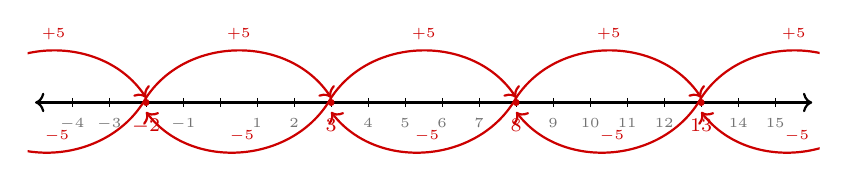
\begin{tikzpicture}[xscale=0.47, yscale=0.5]
  \draw[<->,thick] (-5.0,0) -- (16.0,0);
  \foreach \x in {-4,...,15}{ \draw (\x,0.12) -- (\x,-0.12); }
  \foreach \x in {-4,-3,-1,1,2,4,5,6,7,9,10,11,12,14,15}{ \node[below,font=\tiny,black!55] at (\x,-0.16) {$\x$}; }
  \foreach \x in {-2,3,8,13}{ \fill[red!80!black] (\x,0) circle (2.6pt);
                              \node[below,font=\scriptsize\bfseries,red!80!black] at (\x,-0.18) {$\x$}; }
  % all five hops are the same +5 arc; the outer two run off the edge
  \begin{scope}
    \clip (-5.2,-1.5) rectangle (16.2,1.9);
    \foreach \a/\b in {-2/3}{
       \draw[->,thick,red!80!black] (\a,0.12) to[bend left=55] node[above,font=\tiny]{$+5$} (\b,0.12); }
      \foreach \a/\b in {3/8,8/13}{
       \draw[->,thick,red!80!black] (\a,0.12) to[bend left=55] node[above,font=\tiny]{$+5$} (\b,0.12); }
    \foreach \a/\b in {-7/-2,13/18}{
       \draw[->,thick,red!80!black] (\a,0.12) to[bend left=55] node[above,font=\tiny]{$+5$} (\b,0.12);}
     \foreach \a/\b in {3/-2}{
       \draw[->,thick,red!80!black] (\a,0.12) to[bend left=55] node[above,font=\tiny]{$-5$} (\b,-0.24); }
      \foreach \a/\b in {8/3,13/8}{
       \draw[->,thick,red!80!black] (\a,0.12) to[bend left=55] node[above,font=\tiny]{$-5$} (\b,-0.24); }
    \foreach \a/\b in {-2/-7,18/13}{
       \draw[->,thick,red!80!black] (\a,0.12) to[bend left=55] node[above,font=\tiny]{$-5$} (\b,-0.24);}
  \end{scope}
\end{tikzpicture}
\end{center}

\begin{itemize}
\item<4-6> \textit{Reflexivity}: \greencheck 
\item<5-6> \textit{Symmetry}:  \greencheck    
\item<6> \textit{Transitivity}:     \greencheck \end{itemize}
}

\only<7->{
\begin{mygreenbox}[title=\text{Reference Material: Recall the Definition}]
Let $n$ be a positive integer.  We say that integers $x$ and $y$ are \textbf{congruent modulo n}, and we write 
\[x \equiv y \quad \text{(mod $n$)} \]
if $n | (x-y)$.
\end{mygreenbox}
\vfill 
}
\pause 


\only<8->{
\colorbox{blue!30}{\textbf{Sketch of proof.}} Congruence mod $n$ is an equivalence relation.

We verify the three properties of an equivalence relationship below. 

\begin{itemize}
\item<9-> \textit{Reflexivity}: \; We need to check $xRx$. That is, we need to check $n|(x-x)$. 
\item<10-> \textit{Symmetry}: \; We need to check that if $xRy$ , then $yRx$.  In other words, we need to check that if $n|(x-y)$, then $n|(y-x)$.   
\item<11> \textit{Transitivity}:    We need to check that if $xRy$ and $yRz$ , then $xRz$.   That is, we need to check that if $n|(x-y)$ and $n|(y-z)$, then $n|(x-z)$. 
\end{itemize}
}
\end{frame}


\begin{frame}{Equivalence classes}
%\small 
% \begin{myredbox}[title=Remark (which may help with intuition)]  
%For intuition, note that $x \equiv y$ (mod $n$) if and only if $x$ and $y$ have the same remainder after dividing by $n$.  For example, $4 \equiv 1$ (mod 3).	 
%\end{myredbox}
%\vfill 
\begin{mygreenbox}[title=Definition]
Let $R$ be an equivalence relation on a set $A$ and let $a \in A$.    \\

The \textbf{equivalence class} of $a$, denoted $[a]$, is the set of all elements of $A$ related (by $R$) to $a$.  That is,
\[  [a] = \set{x \in A: xRa}\]
\end{mygreenbox}
\vfill 
\begin{myyellowbox}[title=Example]
The integers can be partitioned into the following equivalence classes
%
\begin{align*}
[0] &= \set{\hdots, -6, -3, 0, 3, 6, \hdots} \\	
[1] &= \set{\hdots, -5, -2, 1, 4, 7, \hdots} \\	
[2] &= \set{\hdots, -4, -1, 2, 5, 8, \hdots} 
\end{align*}
%
under the relation of congruence mod 3.
\end{myyellowbox}

\end{frame}



%\begin{frame}{Example: Equivalence classes mod 3}
%\begin{center}
%\begin{tikzpicture}[scale=0.82]
%  \fill[red!12] (1.5,-3.6) rectangle (2.5,0.4);
%  \foreach \r in {0,1,2,3}{ \foreach \c in {0,1,2}{
%      \pgfmathtruncatemacro{\v}{3*\r+\c}
%      \ifnum\c=2\relax\def\col{red!80!black}\else\def\col{black!70}\fi
%      \node[font=\small, text=\col] at (\c,-\r) {$\v$};}}
%  \foreach \c in {0,1,2}{ \node[font=\scriptsize\bfseries,black!60] at (\c,0.75) {$[\c]$};
%   		\node[font=\small,black!45] at (\c,-3.9) {$\vdots$}; 
%   		
%   		}
%   		
%  \draw[red!70,thick] (1.5,-3.6) rectangle (2.5,0.4);
%\end{tikzpicture}
%\end{center}
%\vfill 
%\begin{center}
%\begin{tikzpicture}[xscale=0.62]
%  \draw[thick] (-3.4,0) -- (12.4,0);
%  \node[font=\small,black!55] at (-4.1,0) {$\cdots$};
%  \node[font=\small,black!55] at (13.1,0) {$\cdots$};
%  \foreach \x in {-3,...,12}{ \draw (\x,0.12) -- (\x,-0.12); }
%  \foreach \x in {-3,-2,0,1,3,4,6,7,9,10,12}{ \node[below,font=\tiny,black!55] at (\x,-0.16) {$\x$}; }
%  \foreach \x in {-1,2,5,8,11}{ \fill[red!80!black] (\x,0) circle (2.6pt);
%                                \node[below,font=\scriptsize\bfseries,red!80!black] at (\x,-0.18) {$\x$}; }
%  \foreach \a/\b in {-1/2,2/5,5/8,8/11}{
%     \draw[->,thick,red!80!black] (\a,0.12) to[bend left=55] node[above,font=\tiny]{$+3$} (\b,0.12); }
%\end{tikzpicture}
%\end{center}
%\end{frame}

\begin{frame}
\footnotesize 
\begin{myredbox}[title=Remark]
\textbf{Q:} Why do equivalence relations matter?  \\
\textbf{A:} They can make problem solving easier.
\end{myredbox}

\vfill
\begin{mygreenbox}[title=Example]
\textbf{Q:} Why is $n^{70} - n^{22}$ always even? \\

\pause 
\textbf{Useful Point-Of-View (POV):} Let us define the "mod-2" equivalence relation (written $\equiv_2$).  Here two numbers are equivalent if they have the same remainder when divided by 2. \pause  So
%
\begin{align*}
	x  \equiv_2 
	\begin{cases}
0, & \text{ if $x$ is even} \\
1, & \text{ if $x$ is odd}
	\end{cases}
\end{align*}
%
%(That is, all even numbers are equivalent to 0 and all odd numbers are equivalent to 1.)  \\
\pause Now multiplication and addition is well-defined mod-2. (For justification, see Hampkins Ch2.) This means we can just use "0" and "1" as representatives in any multiplication or addition problem about odds and evens. \\

\pause 
\textbf{A:} By the above POV, we only need to consider two cases:
\begin{align*}
	n^{70} - n^{22} &= 0^{70} - 0^{22} =0-0 = 0 && \text{ if $n=0$ ($n$ is even)}\\
	n^{70} - n^{22} &= 1^{70} - 1^{22} =1-1 = 0 && \text{ if $n=1$ ($n$ is odd)}
\end{align*}
Either way, the result is 0 (the result is even).

\end{mygreenbox}

\end{frame}



%\begin{frame}{Proving equivalence relations}
% \begin{myredbox}[title=Practice Reading Quiz (Equivalence Relations) ]  
% Prove the theorem below. 
%\end{myredbox}
%\vfill 
%\begin{myyellowbox}[title=Theorem]
%Let $n$ be a positive integer.  Congruence modulo $n$ is an equivalence relation on the set of integers.
%\end{myyellowbox}
%\vfill 
%\begin{mygreenbox}[title=Recall the Definition]
%Let $n$ be a positive integer.  We say that integers $x$ and $y$ are \textbf{congruent modulo n}, and we write 
%\[x \equiv y \quad \text{(mod $n$)} \]
%if $n | (x-y)$.
%\end{mygreenbox}
%\vfill 
%%\textbf{Remark.} For intuition, note that $x \equiv y$ (mod $n$) if $x$ and $y$ have the same remainder after dividing by $n$.  For example, $6 \equiv 1$ (mod 5).
%\end{frame}









\begin{frame}[standout]
Group exercises
\end{frame}

\begin{frame}
\begin{columns}
\begin{column}{0.33\textwidth}
Ashley, Isabelle: 7 \\ 
Bailey, Tanna: 8 \\ 
Blaisdell, Olyver: 2 \\ 
Brown, Ashton: 11 \\ 
Brown, Jonathan: 5 \\ 
Cardenas, Dominic: 4 \\ 
Cutler, George: 8 \\ 
Fabik, Roland: 12 \\ 
Fellows, Audrey: 4 \\ 
Fitzgerald, Ryan: 10 \\ 
Fuller, Ryan: 11 \\ 
Griffen, Clara: 6 \\ 
Grutsch, Tanner: 10 \\\end{column}
\begin{column}{0.33\textwidth}
Hager, Nathan: 6 \\ 
Horner, Jayden: 9 \\ 
Johnson, Jaret: 4 \\ 
Kintzel, Samantha: 13 \\ 
Lameres, Alexis: 2 \\ 
Lee, Holden: 3 \\ 
Mayala, Reece: 5 \\ 
McLean, Connor: 6 \\ 
Mcbride, Daniel: 8 \\ 
Miller, Maverick: 12 \\ 
Moss, Emily: 5 \\ 
Mousseau, Matthew: 12 \\ 
Neuman, Evan: 1 \\\end{column}
\begin{column}{0.33\textwidth}
Putnam, John: 3 \\ 
Ramos, Vydel: 11 \\ 
Rathbun, Jedidiah: 2 \\ 
Roberts, Matthew: 1 \\ 
Roller, Nathan: 13 \\ 
Ryan, Otis: 10 \\ 
Shevtsov, Timothy: 13 \\ 
Sinclair, Aidan: 3 \\ 
Smith, Charles: 7 \\ 
Stensland, Emma: 9 \\ 
Thiessen, Logan: 1 \\ 
Thompson, Jaiden: 9 \\ 
Vath, Ethan: 7 \\\end{column}
\end{columns}
\end{frame}



\begin{frame}{Group exercises}
\small
\begin{enumerate}
	\item Which of the following are equivalence relations?
	\begin{itemize} \footnotesize 
	\item[a.] $|$ on $\mathbb{Z}$.
	\item[b.] $\leq$ on $\mathbb{Z}$.
	\item[c.] Is-an-angram-of on the set of English words. (For instance, \texttt{STOP} is an anagram of \texttt{POTS} because we can form one from the other by rearranging its letters.)
	\item[d.] $R=\set{(1,2),(2,3),(3,1)}$ on the set $\set{1,2,3}$.
	\item[e.] $\set{1,2,3} \times \set{1,2,3}$ on the set $\set{1,2,3}$.
	\item[f.] $\set{1,2,3} \times \set{1,2,3}$ on the set $\set{1,2,3,4}$.
	\end{itemize}
	\item For each equivalence relation below, find the requested equivalence class(es).
	\begin{itemize} \footnotesize 
	\item[a.] $R=\set{(1,1), (1,2), (2,1), (2,2), (3,3), (4,4)} $ on $\set{1,2,3,4}$. Find $[1],[2],[3],[4]$
	\item[b.] $R$ is has-the-same-tens-digit on the set $\set{x \in \mathbb{Z} : 100 < x < 200}$.  Find [123].
	\item[c.] $R$ is has-the-same-parents-as on the set of all human beings.  Find [you].
	\item[d.] $R$ is has-the-same-size-as on $2^{\set{1,2,3,4,5}}$.  Find $[\set{1,3}]$.
	\end{itemize}
\item Let $n$ be a positive integer.  Prove that congruence modulo $n$ is an equivalence relation on the set of integers.
%\item Prove Proposition 15.11:  Let $R$ be an equivalence relation on the set $A$ and let $a,x,y \in A$. If $x,y \in [a]$, then $xRy$.
\end{enumerate}
	
\end{frame}


\begin{frame}{Solution to group exercise \#1}
\footnotesize 
\textbf{Problem.} Which of the following are equivalence relations?
	\begin{itemize} \footnotesize 
	\item[a.] $|$ on $\mathbb{Z}$.
	\item[b.] $\leq$ on $\mathbb{Z}$.
	\item[c.] Is-an-angram-of on the set of English words. (For instance, \texttt{STOP} is an anagram of \texttt{POTS} because we can form one from the other by rearranging its letters.)
	\item[d.] $R=\set{(1,2),(2,3),(3,1)}$ on the set $\set{1,2,3}$.
	\item[e.] $\set{1,2,3} \times \set{1,2,3}$ on the set $\set{1,2,3}$.
	\item[f.] $\set{1,2,3} \times \set{1,2,3}$ on the set $\set{1,2,3,4}$.
	\end{itemize}
	\vfill 
\textbf{Solution.}
	\begin{itemize} \footnotesize 
	\item[a.] No, because the relation is not symmetric.  For example, $3R6$ but $6\cancel{R}3$. 
	\item[b.] No, because the relation is not symmetric. For example, $3R4$ but $4\cancel{R}3$. 
	\item[c.] Yes. 
	\item[d.] No, because the relation is not transitive.  In particular, we have $1R2$ and $2R3$, but $1 \cancel{R} 3$.  %(The relation contains $(1,2)$ and $(2,3)$ but not $(1,3).$)
	\item[e.] Yes. 
	\item[f.] No, because the relation is not reflexive. In particular, $4 \cancel{R} 4$. 
	\end{itemize}
	
\end{frame}


\begin{frame}{Solution to group exercise \#2}
\footnotesize 
\textbf{Problem.} For each equivalence relation below, find the requested equivalence class(es).
	\begin{itemize} \footnotesize 
	\item[a.] $R=\set{(1,1), (1,2), (2,1), (2,2), (3,3), (4,4)} $ on $\set{1,2,3,4}$. Find $[1],[2],[3],[4]$
	\item[b.] $R$ is has-the-same-tens-digit on the set $\set{x \in \mathbb{Z} : 100 < x < 200}$.  Find [123].
	\item[c.] $R$ is has-the-same-parents-as on the set of all human beings.  Find [you].
	\item[d.] $R$ is has-the-same-size-as on $2^{\set{1,2,3,4,5}}$.  Find $[\set{1,3}]$.
	\end{itemize}
\vfill 
\textbf{Solution.} 
	\begin{itemize} \footnotesize 
	\item[a.] We have $[1]=[2]=\set{1,2}$, $[3]=\set{3}$, and $[4]=\set{4}$.
	\item[b.] We have $[123]=\set{120,121,122,123,124,125,126,127,128,129}$.
	\item[c.] The answer depends on who's answering.  I have one sister named Rachael, so for me, $[\text{me}]=\set{\text{me, Rachael}}$.
	\item[d.] We have 
	\[ [\set{1,3}] = \bigg\{ \set{1,2}, \set{1,3}, \set{1,4}, \set{1,5}, \set{2,3}, \set{2,4}, \set{2,5}, \set{3,4}, \set{3,5}, \set{4,5} \bigg\}.\]
	\end{itemize}
\end{frame}

%
%\begin{frame}{Solution to group exercise \#4}
%\textbf{Problem.}  Prove Proposition 15.11:  Let $R$ be an equivalence relation on the set $A$ and let $a,x,y \in A$. If $x,y \in [a]$, then $xRy$.
%\vfill 
%\textbf{Solution.}. By the definition of equivalence classes (Scheinerman Definition 15.6), we have
%%
%\[ [a] =\set{x \in A : xRa}.\]
%%
%Now by assumption, $x \in [a]$, so we have $xRa$.  Similarly, by assumption, $y \in [a]$, so we have $yRa$.  Since R is an equivalence relation, it is symmetric, and so $yRa \implies aRy$.   Now we have $xRa$ and $aRy$, so by transitivity (which holds since R is an equivalence relation), $xRy$.
%\end{frame}


\begin{frame}{Solution to exercise \#3 (proving an equivalence relation)}
\small 
\pause 
We verify the three properties of an equivalence relationship below. 

\begin{itemize}
\item \textit{Reflexivity}: \pause  We need to check $xRx$. That is, we need to check $n|(x-x)$. In other words, we need to check $n|0$.  By definition of divisibility, we need to check that there is an integer $c$ such that $nc=0$.  This is satisfied by setting $c=0$. \; \greencheck 
\item \textit{Symmetry}:\pause   \; We need to check that if $xRy$ , then $yRx$.  In other words, we need to check that if $n|(x-y)$, then $n|(y-x)$.  Let $n|(x-y)$. Then there is an integer $c$ such that $nc = x-y$.  Hence $n(-c) = y-x$.  So $n|(y-x)$.  \; \greencheck  
\item \textit{Transitivity}:  \pause  We need to check that if $xRy$ and $yRz$ , then $xRz$.   That is, we need to check that if $n|(x-y)$ and $n|(y-z)$, then $n|(x-z)$.  By assumption, there are integers $c$ and $d$ such that $nc=(x-y)$ and $nd=(y-z)$.  Now we write
 	\[ x-z = (x-y) + (y-z) = nc + nd = n(c+d).\]
 	Since $c+d$ is an integer, clearly $n|x-z$. \; \greencheck
\end{itemize}
\end{frame}

\end{document}
